\documentclass[manuscript,screen, 12pt, nonacm]{acmart}
\let\Bbbk\relax % Fix for amssymb clash 
\usepackage{vmlmacros}
\AtBeginDocument{%
  \providecommand\BibTeX{{%
    \normalfont B\kern-0.5em{\scshape i\kern-0.25em b}\kern-0.8em\TeX}}}
\usepackage{outlines}
\setlength{\headheight}{14.0pt}
\setlength{\footskip}{13.3pt}
\title{An Alternative to Pattern Matching, Inspired by Verse}

\author{Roger Burtonpatel}
\email{roger.burtonpatel@tufts.edu}
\affiliation{%
\institution{Tufts University}
\streetaddress{419 Boston Ave}
  \city{Medford}
  \state{Massachusetts}
  \country{USA}
  \postcode{02155}
  }
\begin{document}
  

\section{\VMinus can be compiled to a decision tree}
\label{vminustod}

\subsection{Introducing~\D}
\label{d}

While \VMinus exists for writing programs,~\D exists as the target of
translation and provides a means by which to demonstrate~\VMinus's efficient
cost model. This is because the decision-making construct itself in~\D, the
\it{decision tree}, has an efficient cost model. A decision tree can implement
either pattern matching or~\iffibf while guaranteeing never to repeat a test.
The worst-case cost of evaluating a decision tree is linear in its depth, which
itself linear in the size of the code. This desirable property of decision trees
is half of a space-time tradeoff: when a decision tree is produced by compiling
a~\it{case} expression, there are pathological cases in which the total size of
the tree is exponential in the size of the source code (from~\it{case}). Run
time remains linear, but code size may not be. 

Although decision trees are classically used as an intermediate representation
for compiling~\it{case} expressions, in this work, I~use them as a target for
compiling~\iffibf in~\VMinus. In particular, I~show that equations in~\VMinus
can be compiled to a decision tree. 

\D is a generalization of the trees found in~\citet{maranget}. 

\subsection{\D is a generalization of Maranget's trees} 

\D's syntax is given in Figure~\ref{fig:dsyntax}. Decision trees in~\D are
engineered to look like Maranget's trees. 
  
      
  The heart of a decision tree is the~\it{test} form: it takes a value, examines
  it, and chooses a branch based on its form (Maranget calls the operation
  \textsc{Switch}). 

  Let's look at an example from~\citet{maranget} which shows the structure of a
  simple pattern-matching function and its corresponding decision tree. I show
  Maranget's example for two reasons: First, the example serves to bolster your
  understanding of decision trees with a classic, well-established model.
  Second, since I currently have no visualization generator for~\D (\D~can
  currently only be visualized as plain text), I use Maranget's example to have
  a reasonable visual representation of decision trees. The example beings with
  the function,~\tt{merge}, which merges two lists: 

  \begin{figure}[H]
      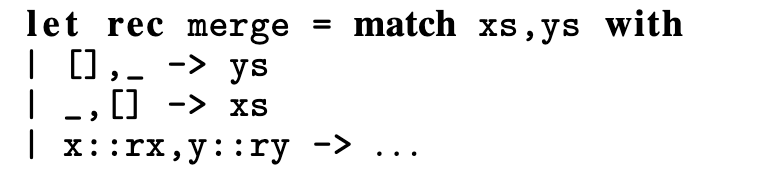
\includegraphics[scale=0.7]{../images/merge.png}
      \Description{Maranget's merge implementation}
      \caption{The skeleton of Maranget's~\tt{merge}}
  \end{figure}

  % He then shows an intermediate representation in his compilation algorithm,
  % the occurrence vector and clause matrix: 

  %~\begin{figure}[H]
  %     \begin{gather*}
  %         \vec{o} = (\tt{xs ys})~\hspace{3em}
  %         P~\rightarrow A = 
  %         \begin{pmatrix}
  %            ~\tt{[]}     &~\tt{\_}     &~\rightarrow~\tt{xs}~\\
  %            ~\tt{\_}     &~\tt{[]}     &~\rightarrow~\tt{ys}~\\
  %            ~\tt{\_::\_} &~\tt{\_::\_} &~\rightarrow~\tt{...} 
  %         \end{pmatrix}
  %     \end{gather*}


  %     \Description{Occurrence vector of names, and clause matrix of matches}
  %     \caption{The occurrence vector and clause matrix are intermediate
  %     representations in Maranget's compilation. I~do not exploit this
  %     representation in my own algorithm, but it helps to understand his final
  %     tree.}
  %~\end{figure}

  The function is compiled to this decision tree: 

  \begin{figure}[H]
      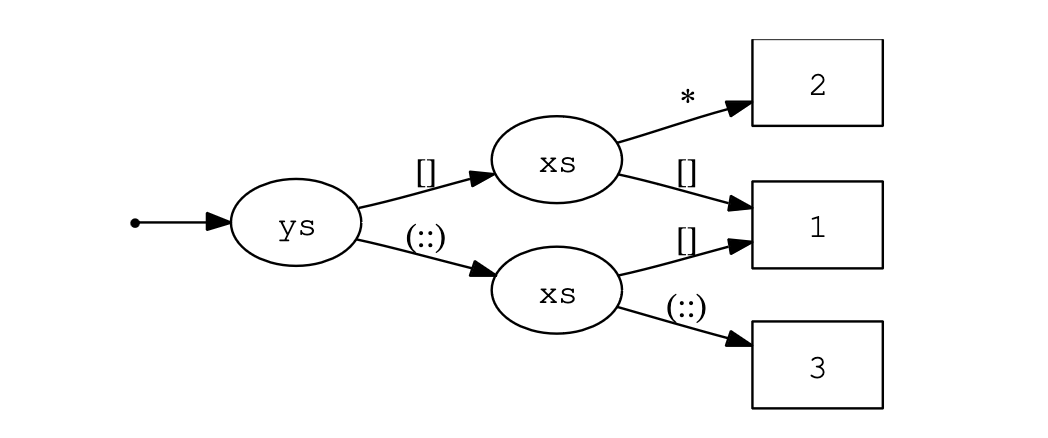
\includegraphics[scale=0.7]{../images/dtree.png}
      \Description{The final decision tree for merge} 
      \caption{The final compiled decision tree for~\tt{merge}, right-to-left}
  \end{figure}

 The decision tree for~\tt{merge}, like the original function, tests values and
 makes decisions. When presented with the values~\tt{xs} and~\tt{ys}, the tree
 first tests ~\tt{xs} against its two known possible forms: the nullary list
 constructor ~\tt{[]}, and an application of the~\it{cons} constructor~\tt{::}.
 If ~\tt{xs} is equal to~\tt{[]}, the tree immediately returns~\tt{ys}. If
 ~\tt{xs} is an application of~\tt{::}, the tree then tests~\tt{ys}
 against~\tt{[]} and~\tt{::}, and it returns a value according to the result of
 the match. Each time the tree goes down a~\tt{::} branch, it extracts the
 arguments of the~\tt{::} for later use: these are~\tt{x}, ~\tt{y},~\tt{xr},
 and~\tt{yr}, which are used in the~\tt{...} branch. This process of extracting
 arguments generalizes to all value constructors with one or more arguments. 

  \begin{figure}
    \begin{center}
    \dcsyntax
    \end{center}
    \Description{The concrete syntax of D.}
    \caption{\D: Concrete syntax}
    \label{fig:dsyntax}
    \end{figure}

  % Here is the decision tree for~\tt{merge} in~\D. 

  %~\begin{figure}[H]
  %   \centering
  %     \it{Like the semantics, this figure is in progress.}
  %     \Description{The decision tree for merge, now in D} 
  %     \caption{The tree for~\tt{merge} in D looks similar to Maranget's.}
  %~\end{figure}

  In~\D, as in Maranget's trees, the~\it{test} node extracts all names from a
  value constructor at once for use in subtrees. The compiler is responsible for
  introducing the fresh names used in~\it{test}. The compiler alpha-renames all
  necessary terms before it translates an~\iffibf to a decision tree to ensure
  all names are unique. 

  In~\D, like in~\VMinus, expressions can~\it{fail}, meaning some of~\D's
  syntactic forms like~\it{try-let} and~\it{cmp} have an extra branch which is
  executed if the examined expression fails. 

    % Includes subsection
    \label{dsemantics}
    \dsemantics


    \subsection{The~\DTran\ algorithm:~\VMinus $\rightarrow$~\D}

    To demonstrate that~\VMinus has a similarly-desirable cost model to pattern
    matching, I~present an algorithm for compiling~\VMinus to a decision tree. I
    choose the decision tree as a target for compilation for the simple reason
    of its appealing cost model. A decision tree can be exponential in size but
    never examines any word of the~\it{scrutinee}---the value being tested---%
    more than once. This property is established by the compilation from~\VMinus
    to \D, which ensuring that no~\it{test} node~\it{T} has any proper ancestor
    \it{T'} such that~\it{T} and~\it{T'} both test the same location in memory.   

    There are a few minor differences in the algorithm I~use and Maranget's: his
    compilation algorithm is more complex than the one in this paper, and
    involves an intermediate representation of occurrence vectors and clause
    matrices which the algorithm I~present does not use. Maranget uses vectors
    and matrices to express multiple simultaneous matches of values to patterns
    as a single match of a vector with a matrix row. This allows him to run a
    \it{specialization} pass that reduces the number of rows in the matrix,
    ultimately leading to smaller trees. Because the trees produced by my
    algorithm still have the linear-in-code-size property, I find them
    acceptable for the current work. 

    The algorithm runs during~\DTran, the transformation from~\VMinus to~\D. Its
    domain, instead of a~\it{case} expression, is~\VMinus's~\iffibf.
    \DTran~propagates a context~\ctx\ which maps each defined name to~\it{known} or
    \it{unknown}. The context is used when determining the form of a guard.
    % in the compilation rules. 
       

    %~\algrenewcommand\algorithmicwhile{\bf{let }}
    %~\algrenewcommand\algorithmicdo{\bf{in }}
    %~\algrenewcommand\algorithmicend{\bf{end}}
    %~\newcommand\alet\algorithmicwhile
    %~\newcommand\ain\algorithmicdo
    %~\newcommand\aend\algorithmicend

    %~\newcommand\branches{\ensuremath{\mathit{branches}}}
    %~\newcommand\mg{\ensuremath{-}}


    When presented with an~\iffibf,~\DTran\~invokes~\Compile with context~\ctx.
    \Compile~first desugars the~\iffibf by expanding choice to multiple~\iffibf
    branches with a desugaring function~\ITran: 
    
    \itran{if\;~\dots~\dbar\; gs_{1};\;~\choiceg{gs_{2}}{gs_{3}};\; gs_{4}~\rightarrow e\;~\dbar~\dots~\;fi}
    
    ==
    
    ${if\;~\dots~\dbar\; gs_{1};\; gs_{2}~\rightarrow e~\;\dbar\; gs_{3};\; gs_{4}~\rightarrow e~\;\dbar~\dots~\;fi}$

    With the desugared~\iffibf,~\Compile\ then repeatedly chooses a guarded
    expression $G$ and applies one of the compilation rules below. The rules are
    applied in a nondeterministic order. 

    The algorithm terminates when it inserts a final~\it{match} node (with rule
    \textsc{Match}).  A~\it{match} node is inserted for a right-hand side expression~\expr when the list of
    guards preceding~\expr is empty or a list of assignments from names to
    unbound names. Termination of~\DTran\~is guaranteed because each recursive
    call passes a list of guarded expressions in which the number of guards is
    strictly smaller, so eventually the algorithm reaches a state in which the
    first unmatched branch is all trivially-satisfied guards.


    If~\Compile\ cannot choose a $g$ of
    one of the valid forms, it halts with an error. This
    can happen when no $g$ is currently solvable in the context, as determined
    by the same algorithm that~\VMinus uses to pick a guard to solve, or when
    the program would be forced to unify incompatible values, such as any value
    with a closure. 

      \subsection{Big-step rules for \Compile}
        \compiler

      \subsection{Reduction Strategies}

      In my implementation, I apply the~\textsc{Test} rule before other rules,
      having found in my experiments that this heuristic leads to the smallest trees. A~%
      risk of inserting a \it{test} node before a \it{let-unless} node is that
      if there are many shared names across branches, a \it{test} node
      will introduce those names in \it{let-unless} nodes in each
      subtree.
      It is possible to insert \it{let-unless} nodes before \it{test}
      nodes, in which case those names will be bound
      only once.  The risk of the \it{let}-first strategy
      is that if there are many names used in only one subtree of a \it{test},
      these names will be introduced to \it{all} branches.  The extra
      bindings may harm
      performance by bloating an environment in an interpreter or thrashing the
      icache if the tree further is compiled to machine code. 

      In the implementation,~\DTran\~first introduces all the names under the
      all existential $\exists$'s to a context which determines if a name is
      \it{known} or~\it{unknown}, applying the~\textsc{Exists} rule is applied
      all at the start. At the start of compilation, each name introduced by
      $\exists$ is~\it{unknown} in a context~\ctx. Since all names in the
      program are unique at this stage, there are no clashes. 

      \subsection{Full Big-step rules for \Compile, with no descriptions}

        The judgement form for compilation is \textsc{Compile}: 

        \showvjudgement{Compile}{\compilebig}

The rules are nondeterministic: the structure of the final result~\expr\ depends
on the order in which rules are applied by the compiler.  

\rawcompiler

    \subsection{Translation from~\VMinus to~\D preserves semantics}
    
    Translating~\iffibf to a decision tree should preserve semantics:
    \begin{conjecture}
      \text{Given a specific but arbitrarily chosen environment~\Rho\; and context~\ctx, when}
      \vmeval[result={\result[1]}]\;and\;\compilebig[iffi=\expr,
      compiled=\expr']\;and\;\vmeval[exp=\expr', result={\result[2]}], then
      {\result[1]} = {\result[2]}. 
    \end{conjecture}
    Proving this conjecture is the subject of future work. 

\end{document}
